\documentclass[letterpaper,8pt,twocolumn,twoside,]{pinp}

%% Some pieces required from the pandoc template
\providecommand{\tightlist}{%
  \setlength{\itemsep}{0pt}\setlength{\parskip}{0pt}}

% Use the lineno option to display guide line numbers if required.
% Note that the use of elements such as single-column equations
% may affect the guide line number alignment.

\usepackage[T1]{fontenc}
\usepackage[utf8]{inputenc}

% pinp change: the geometry package layout settings need to be set here, not in pinp.cls
\geometry{layoutsize={0.95588\paperwidth,0.98864\paperheight},%
  layouthoffset=0.02206\paperwidth, layoutvoffset=0.00568\paperheight}

\definecolor{pinpblue}{HTML}{185FAF}  % imagecolorpicker on blue for new R logo
\definecolor{pnasbluetext}{RGB}{101,0,0} %


\usepackage{booktabs}
\usepackage{longtable}
\usepackage{array}
\usepackage{multirow}
\usepackage{wrapfig}
\usepackage{float}
\usepackage{colortbl}
\usepackage{pdflscape}
\usepackage{tabu}
\usepackage{threeparttable}
\usepackage{threeparttablex}
\usepackage[normalem]{ulem}
\usepackage{makecell}
\usepackage{xcolor}

\title{A multi-variate prediction model to determine housing prices in
New York}

\author[]{Ethan Yong, Sandithi Lewanda, Bradon Holland, Michael Nguyen,
Dan Mahesh}


\setcounter{secnumdepth}{5}

% Please give the surname of the lead author for the running footer
\leadauthor{}

% Keywords are not mandatory, but authors are strongly encouraged to provide them. If provided, please include two to five keywords, separated by the pipe symbol, e.g:
 \keywords{  Github -
\url{https://github.com/ethanyongg/Predicting-NYC-House-Prices}  }  

\begin{abstract}
Abstract: This report aims to analyze the key predictors that impact New
York Housing prices. By assuming there is a linear relationship between
price and predictors, the step-wise regression selection method using
the Akaike information criterion was used to select the best predictors.
The model was iteratively checked by transforming the model to have log
features to meet all linearity assumptions. Subsequently,
multicollinearity checks were used to determine the ultimate model and
ensure model stability. It was found that the key variables impacting
the prices of New York were living area, land value, waterfront, new
construct, heating type, lot size, central air, age, rooms and
bathrooms. However, the analysis is limited as the model may not be
useful beyond 2006, the data has biases, significant predictors of house
prices were not originally included in the dataset, and non-parametric
tests may be required due to some assumption violation.
\end{abstract}

\dates{This version was compiled on \today} 


% initially we use doi so keep for backwards compatibility
% new name is doi_footer
\doifooter{\url{https://github.com/ethanyongg/Predicting-NYC-House-Prices}}


\begin{document}

% Optional adjustment to line up main text (after abstract) of first page with line numbers, when using both lineno and twocolumn options.
% You should only change this length when you've finalised the article contents.
\verticaladjustment{-2pt}

\maketitle
\thispagestyle{firststyle}
\ifthenelse{\boolean{shortarticle}}{\ifthenelse{\boolean{singlecolumn}}{\abscontentformatted}{\abscontent}}{}

% If your first paragraph (i.e. with the \dropcap) contains a list environment (quote, quotation, theorem, definition, enumerate, itemize...), the line after the list may have some extra indentation. If this is the case, add \parshape=0 to the end of the list environment.


\section{Introduction}\label{introduction}

Access to quality, affordable housing is fundamental to well-being.
Hence this report aims to help New York property valuation companies
make fair pricing decisions by analysing the intrinsic features of
houses. It is initially hypothesised that factors like lot size,
waterfront features, and age are the most important factors that shape a
house's price.

\section{Data Description}\label{data-description}

The data is classified as secondary data with the features of 1734
houses in Saratoga County, New York, USA in 2006 randomly sampled from a
Saratoga Country directory. It can be assumed that this dataset avoids
non-response bias as it was originally taken from public records from
Saratoga County, based on mandatory tax recording data (Saratoga County,
2006). More biases and limitations will be discussed further below.

The data has 1734 observations and is recorded in wide format with a mix
of quantitative and qualitative 16 variables such as ``price'' and
``lotsize'' recorded per each house.

\subsection{Data Cleaning}\label{data-cleaning}

Dataset was cleaned using tidyverse (Wickham, 2017) by removing dummy
variables, converting categorical variables like waterfront features
into factors to ensure it was captured by the regression model, and
checking for missing values.

\section{Analysis}\label{analysis}

\begin{figure}[h]

{\centering \includegraphics[width=0.7\linewidth]{Report_files/figure-latex/{Heatmap}-1} 

}

\caption{Heatmap of correlations between quantitative variables}\label{fig:{Heatmap}}
\end{figure}

\subsection{Variable Selection}\label{variable-selection}

Backwards stepwise selection was implemented to determine the most
important predictors. Variables in the full model were then subsequently
dropped when measured against the AIC which determines the model with
greatest amount of variation using the least amount of predictors. When
the AIC was lower than the previous model it would be accepted as the
new model; this process would continue until the final model remains.
Implementing the backwards selection resulted in 4 variables being
dropped from the full model (fuel\_type, sewer\_type, pct\_college,
fireplaces).

To validate our findings, a forward model was also performed. This
method started with the null model which initally contained no
variables. Next, the most significant variables were added for each
iteration until the AIC was no longer higher than the previous model.

After comparing the results, it was discovered that the forwards model
was identical to the backwards model which reinforces the validity of
the model. In cases like this the backward model is usually generally
the preferred method as the forward model produces suppressor effects
sometimes. However in this case there is no significance.

\subsection{Assumption Checks for Stepwise Regression
Model}\label{assumption-checks-for-stepwise-regression-model}

\textbf{Independence:} Some independence is already assumed due to the
design of data collection. However, it is expected that this assumption
may be slightly skewed as the price of a house in one area is inevitably
impacted by those around it.

\textbf{Linearity:} While the residual plot (Figure 3) for the Step AIC
model highlighted that points were symmetrically distributed above and
below the zero axis, the scatterplots (Figure 6) of the individual
variables showed that most of the independent variables against
``price'' were severely distorted. To remedy this, quantitative
independent variables were logged.

\textbf{Homoscedasticity:} While most residual data points are randomly
clustered in nature and evenly spaced, there appears to be some form of
heteroscedasticity as the distances between some data points ``fanned
out'' as the fitted values increased(Figure 3). This indicates that for
a few data points, the predicted error value is increasing due to the
presence of outliers.

\textbf{Normality:} From the QQPlot, our normality assumption appears to
be severely violated for the start and end of the axis as seen by the
number of outliers (Figure 3). However, due to the central limit theorem
(\textgreater30 observations), the sample is approximately normal, and
valid inferences can be made.

\subsection{Log Transformation}\label{log-transformation}

To resolve issues with linearity, normality, and homoscedasticity, log
transformations were undertaken on the predictors selected by the AIC
method to create a log-linear (dependent variable was logged) and a
log-log model (both dependent and quantitative independent variables
were logged). Note that the scatterplot highlighted living\_age was
fairly linear and didn't require to be transformed but logging this
variable improved the R\^{}2 from 0.58 to 0.59. The log-log model was
chosen as the final model as it had the highest R\^{}2 value with the
lowest RMSE (Table 3).

\subsection{Checking Correlations}\label{checking-correlations}

Multi-collinearity within independent variables is important to identify
as it may undermine model stability by reducing the precision of the
estimated coefficients. The correlation matrix (Figure 1)showed that the
living area was highly correlated with bedrooms, rooms, and bathrooms.
However, in-sample and out-of-sample performance (Table 1) deteriorated
when all 3 variables were removed but remained stable when only
``bedrooms'' was removed. Further, results for the final model was
confirmed with a AIC criterion selection. Thus, bedrooms was dropped to
establish the final model.

\subsection{Final Assumption analysis}\label{final-assumption-analysis}

Following the development of the final model using log-log
transformation, homogeneity improved with the reduction in the fanning
out of data points (Figure 4). Whilst normality improved as some
residual points were closer to the reference line, some outliers still
exist in the outer edges of the fitted value axis. These outliers could
potentially be explained by high wealth inequality in areas like New
York, leading to few houses having higher prices than most. Whilst
linearity was maintained (symmetrical number of points across zero), the
scatterplot showed transformation only improved for 2 out of the 4
variables (Figure 6 vs 7) highlighting that the linearity assumption is
still slightly violated, indicating that future models may need
non-parametric tests like a kernel regression analysis. The independency
assumption remained the same.

\begin{table}[H]

\caption{\label{tab:unnamed-chunk-3}Comparison table comparing performance when additional variables are removed}
\centering
\begin{tabular}[t]{l|r|r|r}
\hline
  & RMSE & Rsquared & MAE\\
\hline
Without bedrooms, rooms and bathroms & 0.2945 & 0.5849 & 0.2099\\
\hline
without bedrooms & 0.2895 & 0.5967 & 0.2065\\
\hline
with bedrooms & 0.2905 & 0.5941 & 0.2066\\
\hline
\end{tabular}
\end{table}

\subsection{Model Selection}\label{model-selection}

We decided to drop the bedroom variable from the model as its removal
improved RMSE, MAE and \(r^2\) values (Table 3). Furthermore, bedrooms
had a very high correlation value with living area, thus removing it
would reduce multicollinearity.

\section{Results}\label{results}

\subsection{Final Model}\label{final-model}

\begin{equation}
\begin{aligned}
\operatorname{\widehat{log\_price}} &= 7.065 + 0.49(\operatorname{\log\_living\_area})\ + \\
&\quad 0.119(\operatorname{\log\_land\_value}) + 0.549(\operatorname{waterfront}_{\operatorname{True}})\ - \\
&\quad 0.149(\operatorname{new\_construct}_{\operatorname{True}}) + 0.07(\operatorname{heat\_type}_{\operatorname{Hot\ Air}})\ + \\
&\quad 0.051(\operatorname{heat\_type}_{\operatorname{Hot\ Water}}) - 0.403(\operatorname{heat\_type}_{\operatorname{None}})\ + \\
&\quad 0.111(\operatorname{\log\_lot\_size}) + 0.044(\operatorname{central\_air}_{\operatorname{True}})\ - \\
&\quad 0.037(\operatorname{\log\_age}) + 0.011(\operatorname{rooms})\ + \\
&\quad 0.104(\operatorname{bathrooms})
\end{aligned}
\end{equation} The model's \textbf{in-sample performance} was checked
using F-test values, \(R^2\) (explanatory power of independent
variables), and the adjusted \(R^2\) figure. With an F-test value 207.8
the p-value of 2.2 e-16 is less than the significant value of 5\%,
providing sufficient evidence that the final model fits the data better
than a model with no independent variables. The final model's \(R^2\)
analysis was overshadowed by the full model's (no variables removed)
value, assumed due to having more variables. However, the adjusted
\(R^2\) figure for both figures was equivalent (Table 2), indicating the
final model's efficiency.

\begin{table}[H]

\caption{\label{tab:In-sample performances}Comparison table comparing in-sample performance of different transformation techniques}
\centering
\begin{tabular}[t]{l|r|r}
\hline
  & Adjusted R squared & R squared\\
\hline
Final model & 0.589 & 0.592\\
\hline
Initial model & 0.590 & 0.595\\
\hline
Log-Linear & 0.582 & 0.586\\
\hline
Linear-Log & 0.593 & 0.596\\
\hline
\end{tabular}
\end{table}

The model's \textbf{out-of-sample performance} was checked using a
10-fold cross-validation model (Kuhn, 2022) to extract Mean Absolute
Error (MAE) and Root-Squared Mean Error (RMSE). Whilst the final model
had the lowest RMSE and MAE compared to all other models (Table 3), the
differences were marginal except compared to the simple model (simple
linear regression with living\_area which correlated the most with
price). This indicates that the final model predicts the dependent
variable better than the singular independent variables.

Interestingly, the interval of MAE for the selected final model was much
narrower (Figure 2b.) compared to the initial and single model
indicating the strength of the final model- MAE is a much better
evaluation metric for the current model given its power to adjust for
outliers compared to RMSE.

\begin{table}[H]

\caption{\label{tab:Cross Validation}Comparison table comparing performance of different transformation techniques}
\centering
\begin{tabular}[t]{l|r|r|r}
\hline
  & RMSE & Rsquared & MAE\\
\hline
Full Log Model & 0.2917 & 0.5947 & 0.2073\\
\hline
Log-Log Model & 0.2906 & 0.5958 & 0.2071\\
\hline
Log-Linear Model & 0.2923 & 0.5913 & 0.2073\\
\hline
Linear-Log Model & 62948.3428 & 0.5921 & 44855.4845\\
\hline
Simple Model & 0.3301 & 0.4785 & 0.2346\\
\hline
\end{tabular}
\end{table}

\section{Discussion}\label{discussion}

\subsection{Limitations}\label{limitations}

\textbf{1.} The initial data may be subjected to \textbf{measurement
bias} as there is no evidence to probe if all measurement techniques
(i.e lot\_size) were centralised for all houses. Furthermore, the data
may create \textbf{selection bias} as the county of Saratoga is not
representative of the entire state of New York, leading to incorrect
evaluation of predictors impacting housing prices in this state.
\textbf{2.} Due to the inflationary nature of house prices, predictive
model may not be useful for any year beyond 2006. To be of use across
multiple years, the model could be multiplied by a common inflationary
factor. \textbf{3.} The final model presented was fairly weak with an
adjusted R-squared value of 0.59, indicating that either the predictors
had a non-linear or another type of relationship (i.e.~parabolic) with
price or the model required better independent variables. Stronger
extrinsic factors such as macroeconomic variables like interest rates,
distances to schools and jobs could have been integrated into the model.
Further, non-parametric regression models could have been used
considering the slight violation of normality and linearity assumptions.
\textbf{4.} The AIC selection method has limitations like the p-values
being be too low due to multiple comparisons (Harrel, 2001), leading to
erroneous model selection. In the future, model results could be be
compared to other methods like the Bayenesian Information Criteria
(BIC).

\subsection{Conclusion}\label{conclusion}

After removing variables through backwards and forwards elimination
while also removing additional variables due to multicollinearity, our
final model found 10 significant variables that can predict New York
City house prices with an RMSE of 0.2906 and an MAE of 0.2071. For
example, a 1\% change in living area would increase house prices by
0.49\%, holding all other variables constant. A one unit increase in
rooms would lead to a 1.1\% increase in price on average, holding all
other variables constant. An MAE of 0.2071 means that the predictions
and true value may vary by 0.2071. However, our model has an \(r^2\)
value of only 0.5958, meaning only 59.98\% of the variability in house
prices can be explained by our model. There is still room for
improvement for predicting house prices in NYC through the utilization
of other machine learning algorithms.

\section{References}\label{references}

Allaire, J.J., Xie et al.~(2022). rmarkdown: Dynamic Documents for R.
{[}online{]} R-Packages. Available at:
\url{https://CRAN.R-project.org/package=rmarkdown} {[}Accessed 17
Sep.~2022{]}.

ASA Community. (n.d.). Community.amstat.org. Retrieved November 6, 2022,
from \url{https://community.amstat.org/stats101/home} ‌Harrell, F.
(2001). Regression Modeling Strategies {[}Review of Regression Modeling
Strategies{]}.

Max Kuhn. (2022). caret: Classification and Regression Training. R
package version 6.0-93. \url{https://CRAN.R-project.org/package=caret}

Wickham (2017). Easily Install and Load the `Tidyverse' {[}R package
tidyverse version 1.2.1{]}. R-project.org. {[}online{]}
\url{doi:https://CRAN.R-project.org/package=tidyverse}.

Wickham, H., François, R., Henry, L., Müller, K. and RStudio (2020).
dplyr: A Grammar of Data Manipulation. {[}online{]} R-Packages.
Available at:
\url{https://cran.r-project.org/web/packages/dplyr/index.html}. Xie Y
(2022). knitr: A General-Purpose Package for Dynamic Report Generation
in R. R package version 1.40, \url{https://yihui.org/knitr/}.

\newpage

\section{Appendix}\label{appendix}

\begin{figure}[h]

{\centering 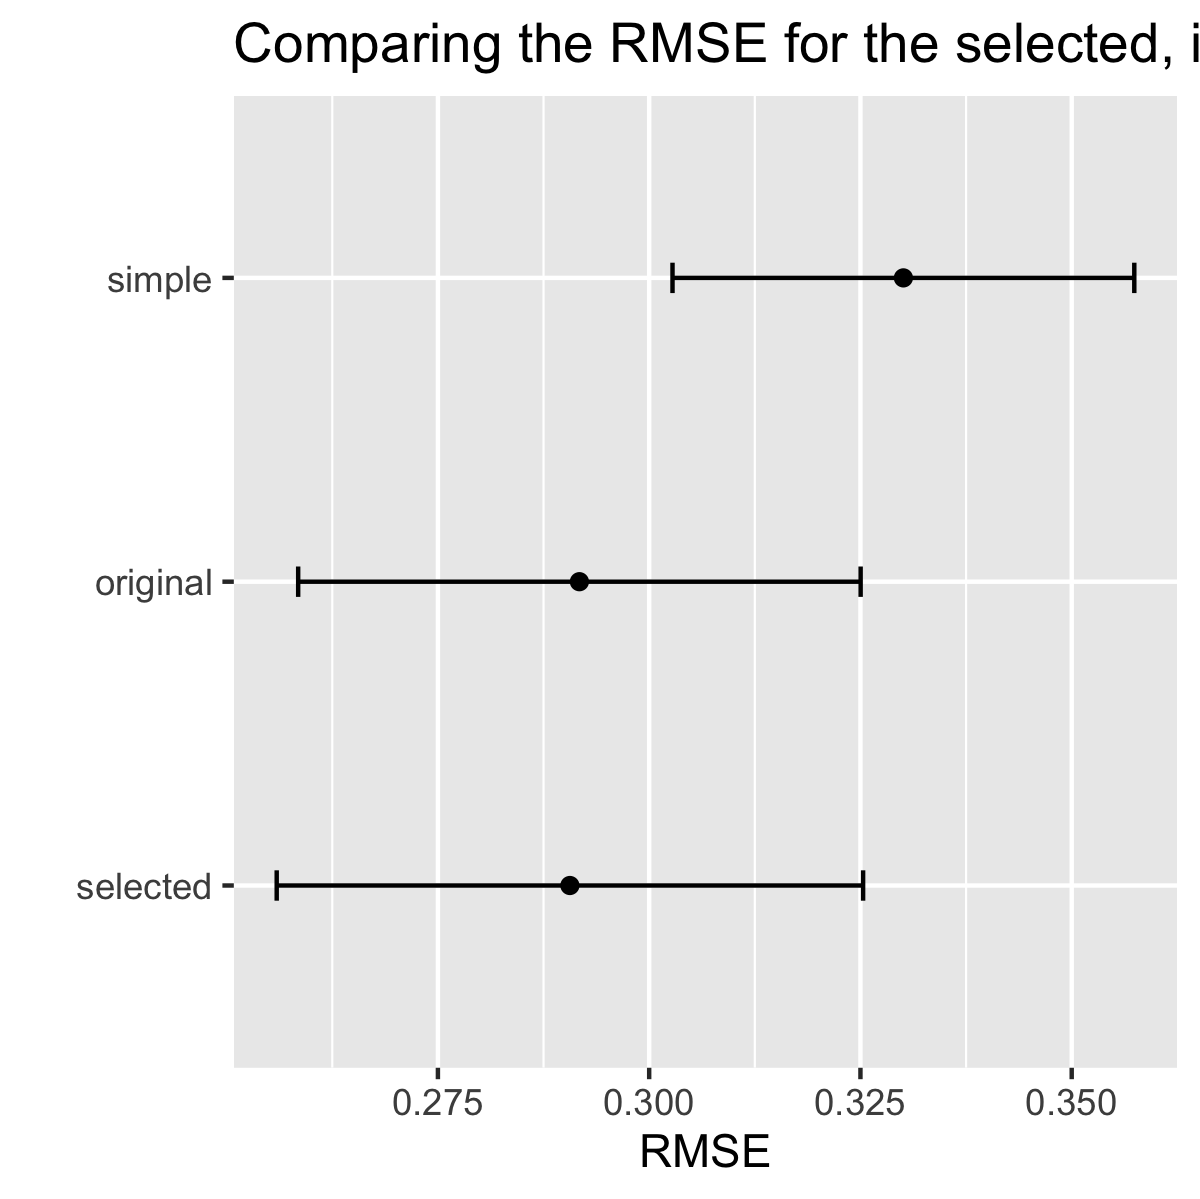
\includegraphics[width=0.49\linewidth]{plot10} 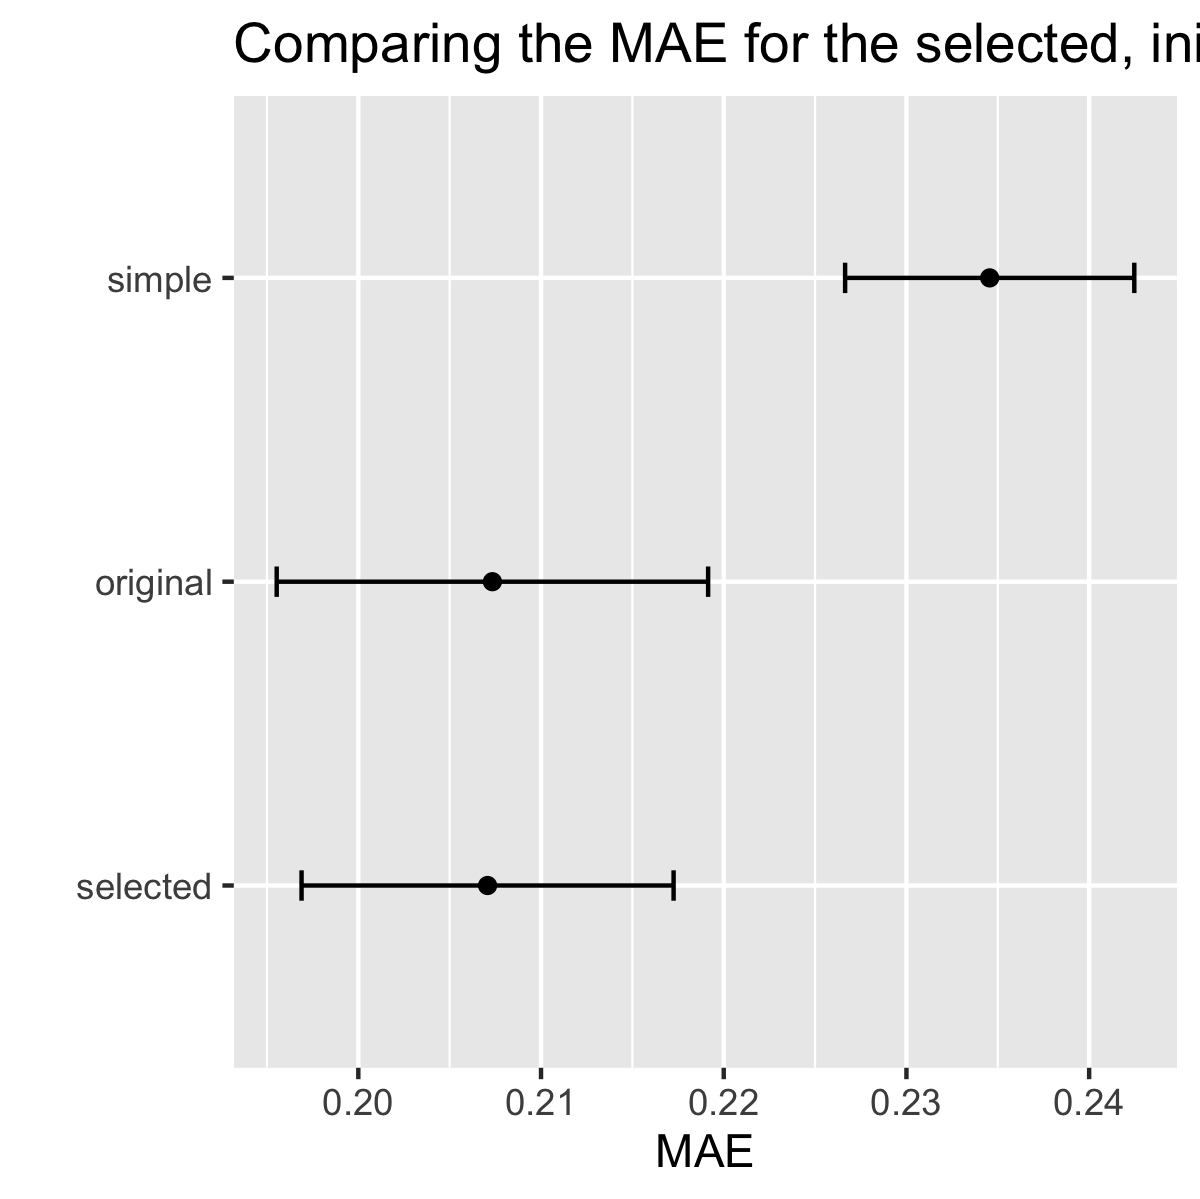
\includegraphics[width=0.49\linewidth]{plot11} 

}

\caption{RMSE and MAE comparison for simple, original and selected models}\label{fig:unnamed-chunk-6}
\end{figure}

\begin{figure}[h]

{\centering 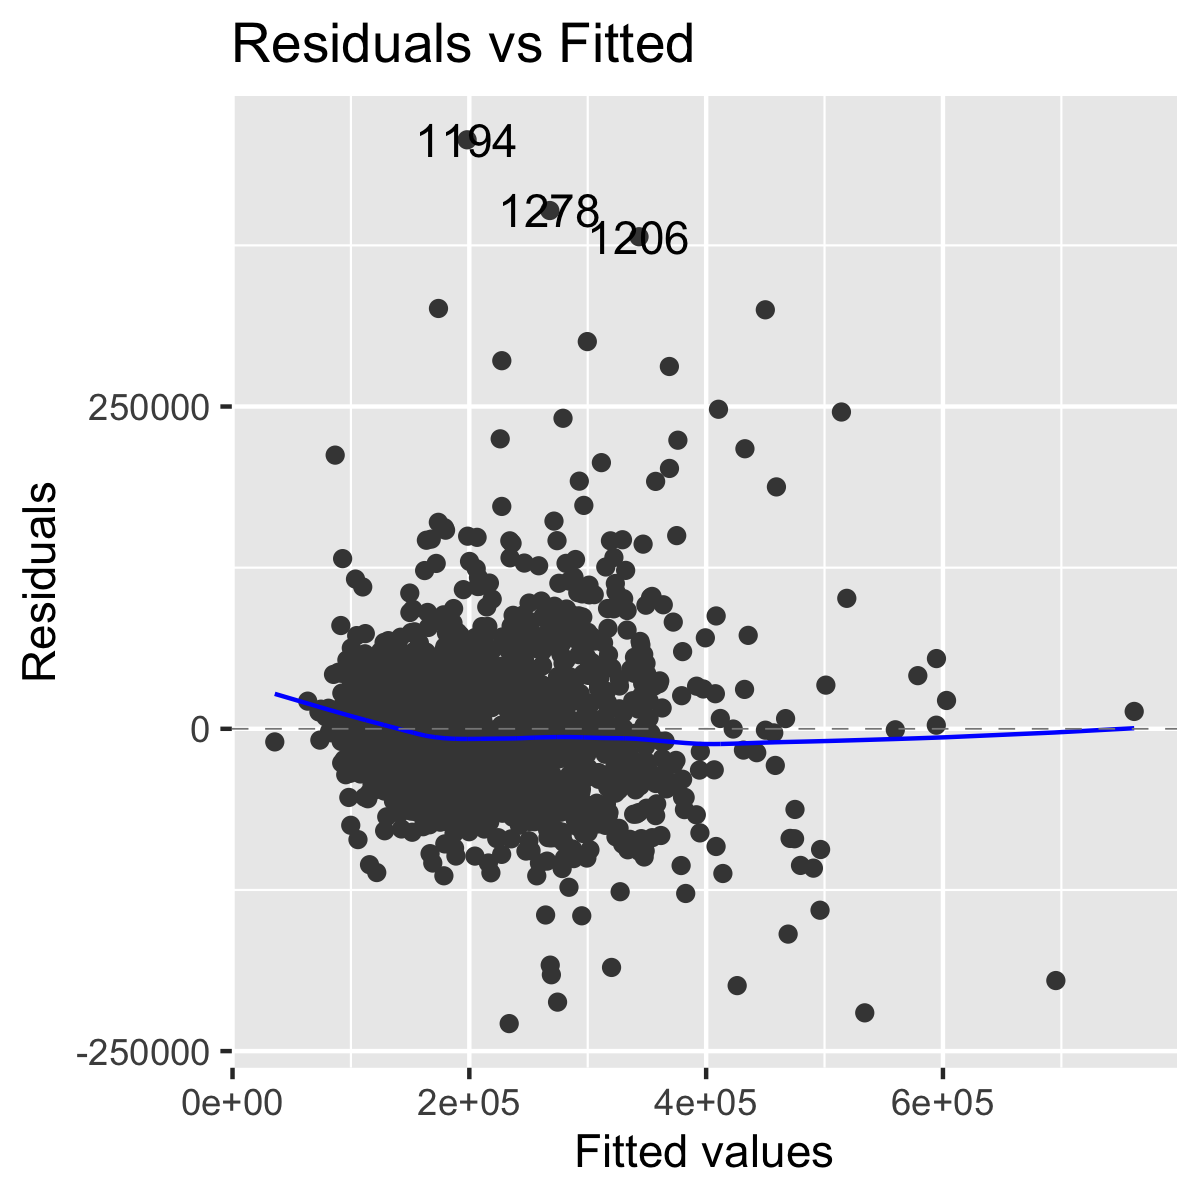
\includegraphics[width=0.49\linewidth]{plot1} 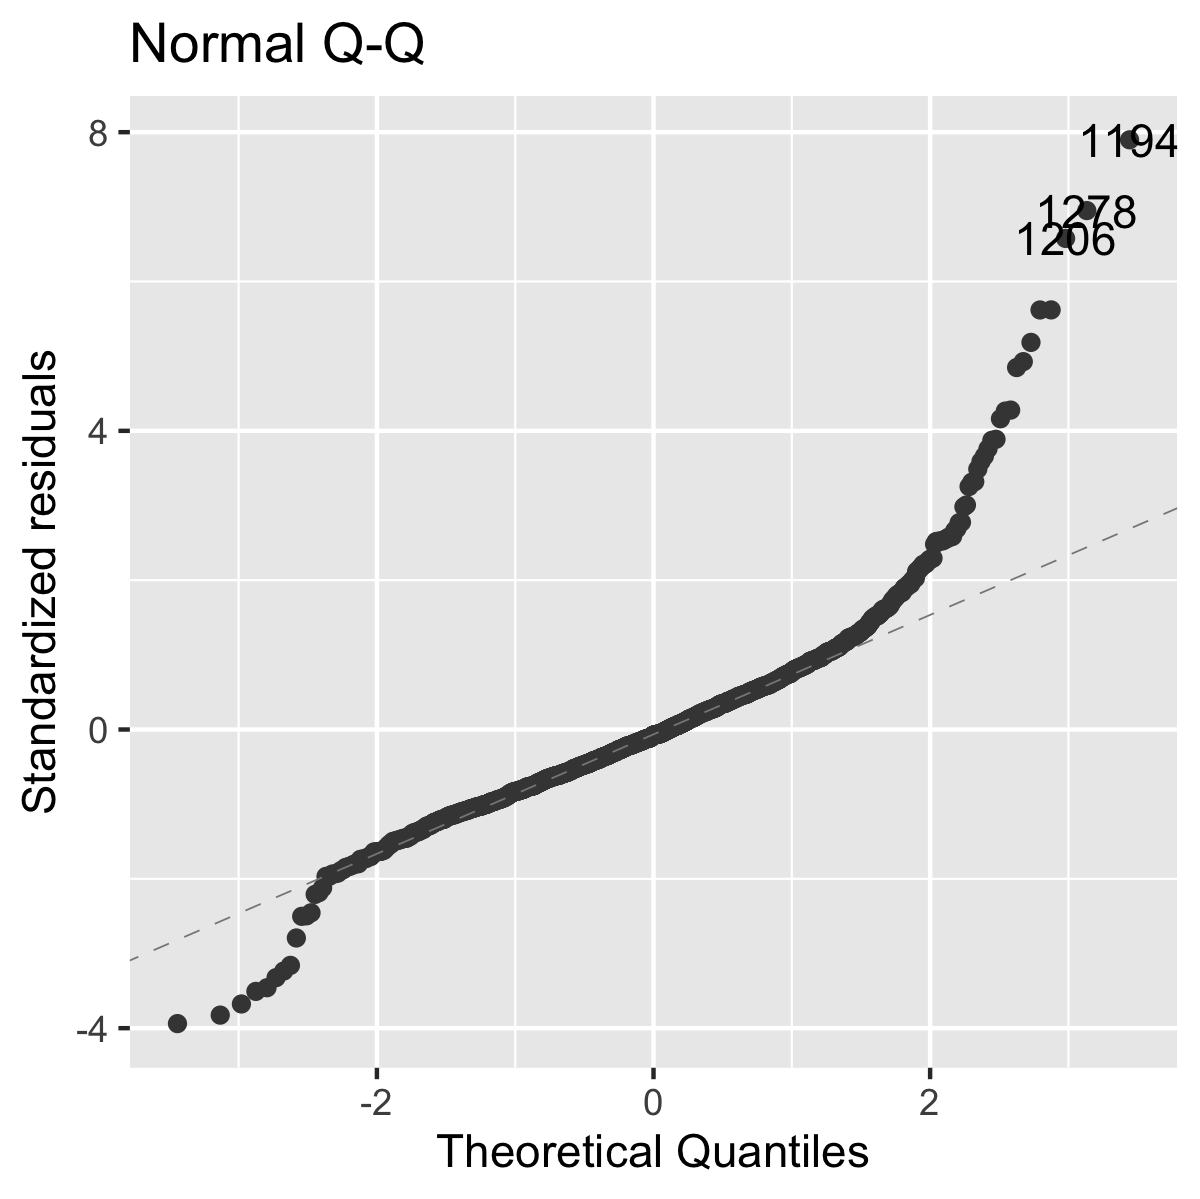
\includegraphics[width=0.49\linewidth]{plot2} 

}

\caption{Residual and QQplot for model selected through AIC method}\label{fig:Assumption check simple}
\end{figure}

\begin{figure}[h]

{\centering 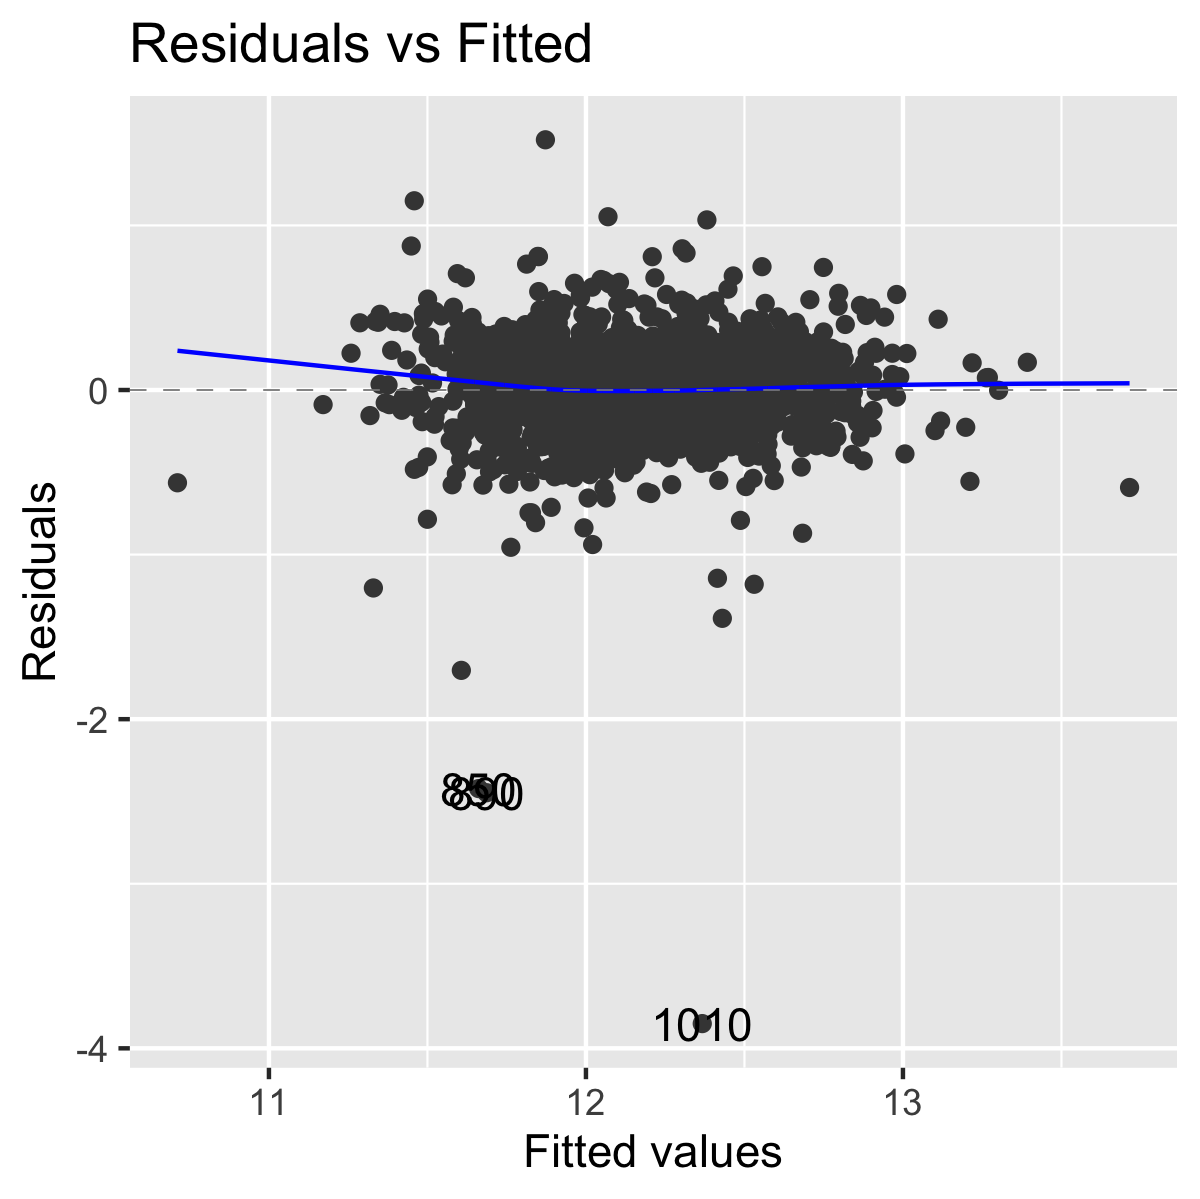
\includegraphics[width=0.49\linewidth]{plot3} 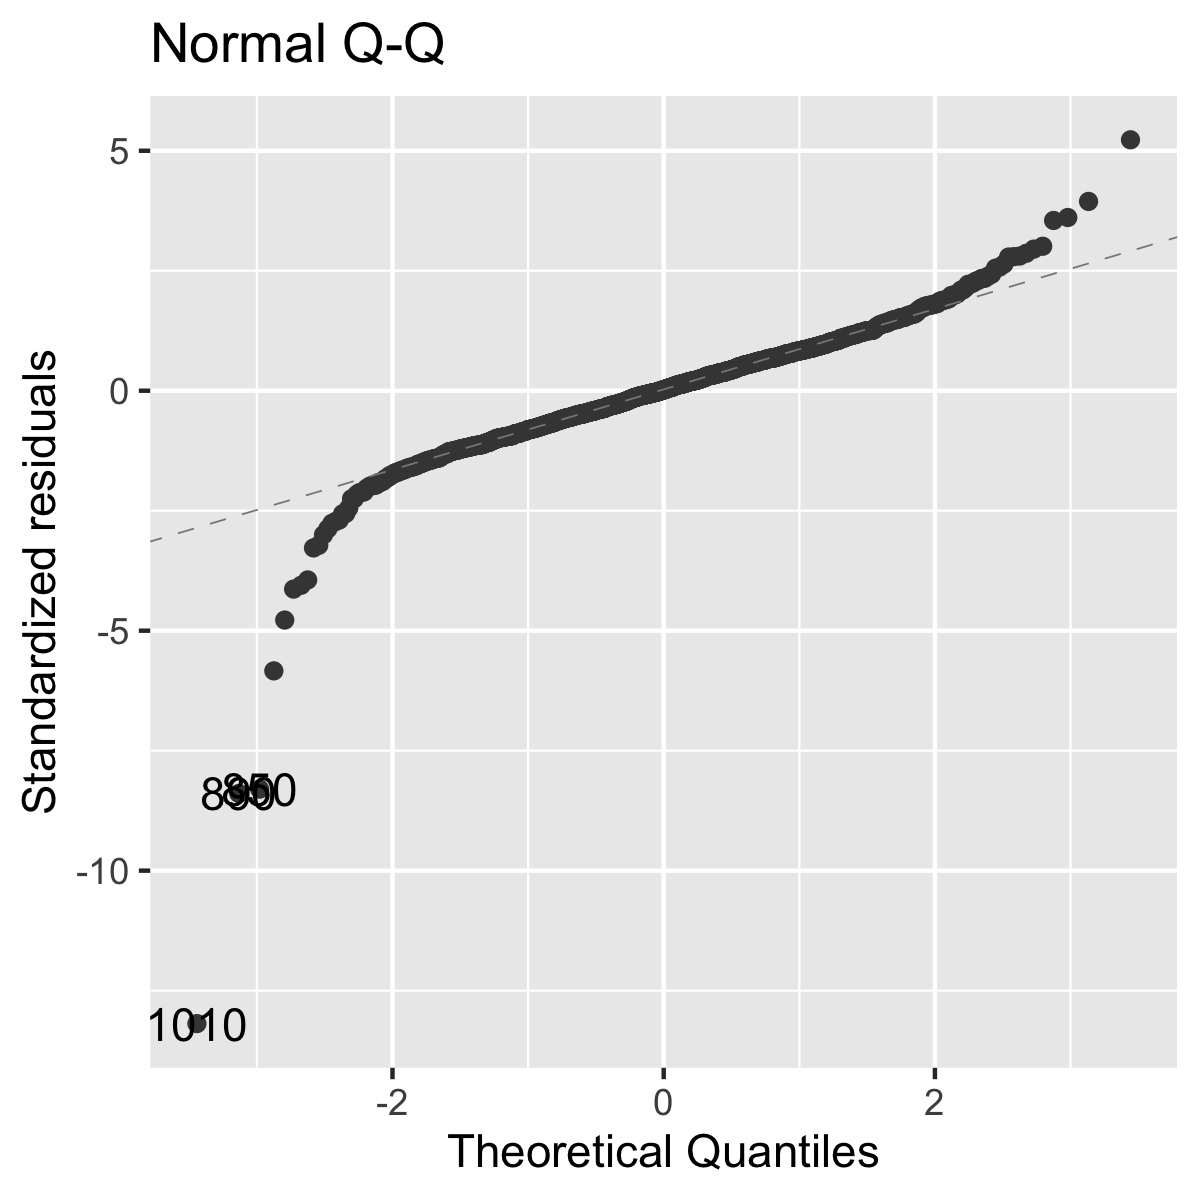
\includegraphics[width=0.49\linewidth]{plot4} 

}

\caption{Residual vs Fitted and QQplot for log-log transformed model}\label{fig:log-log assumption}
\end{figure}

\begin{figure}[h]

{\centering 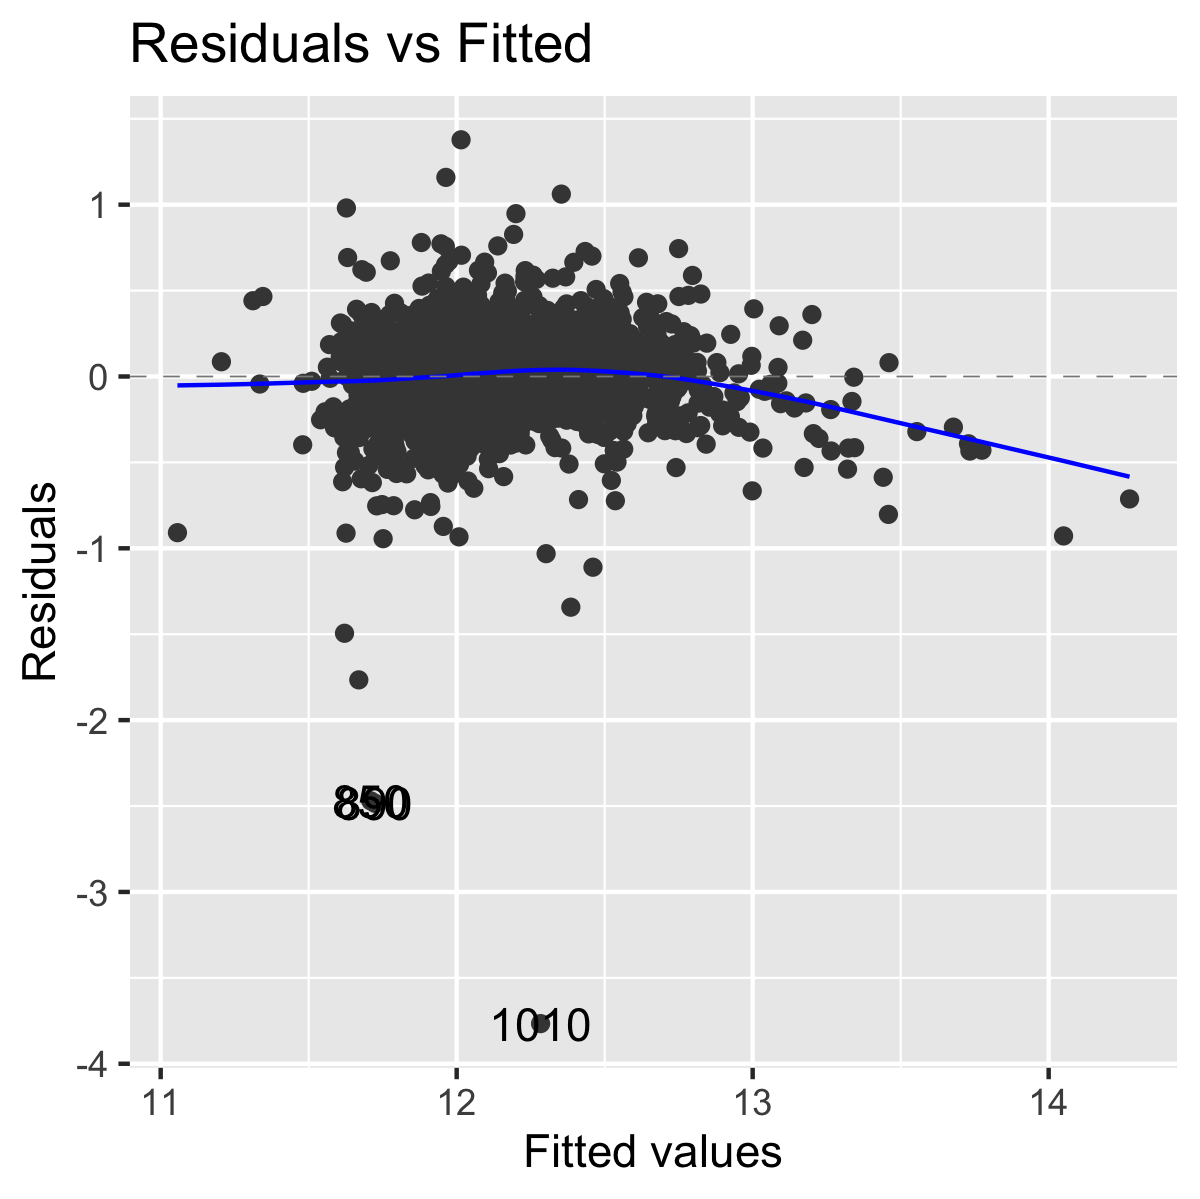
\includegraphics[width=0.49\linewidth]{plot5} 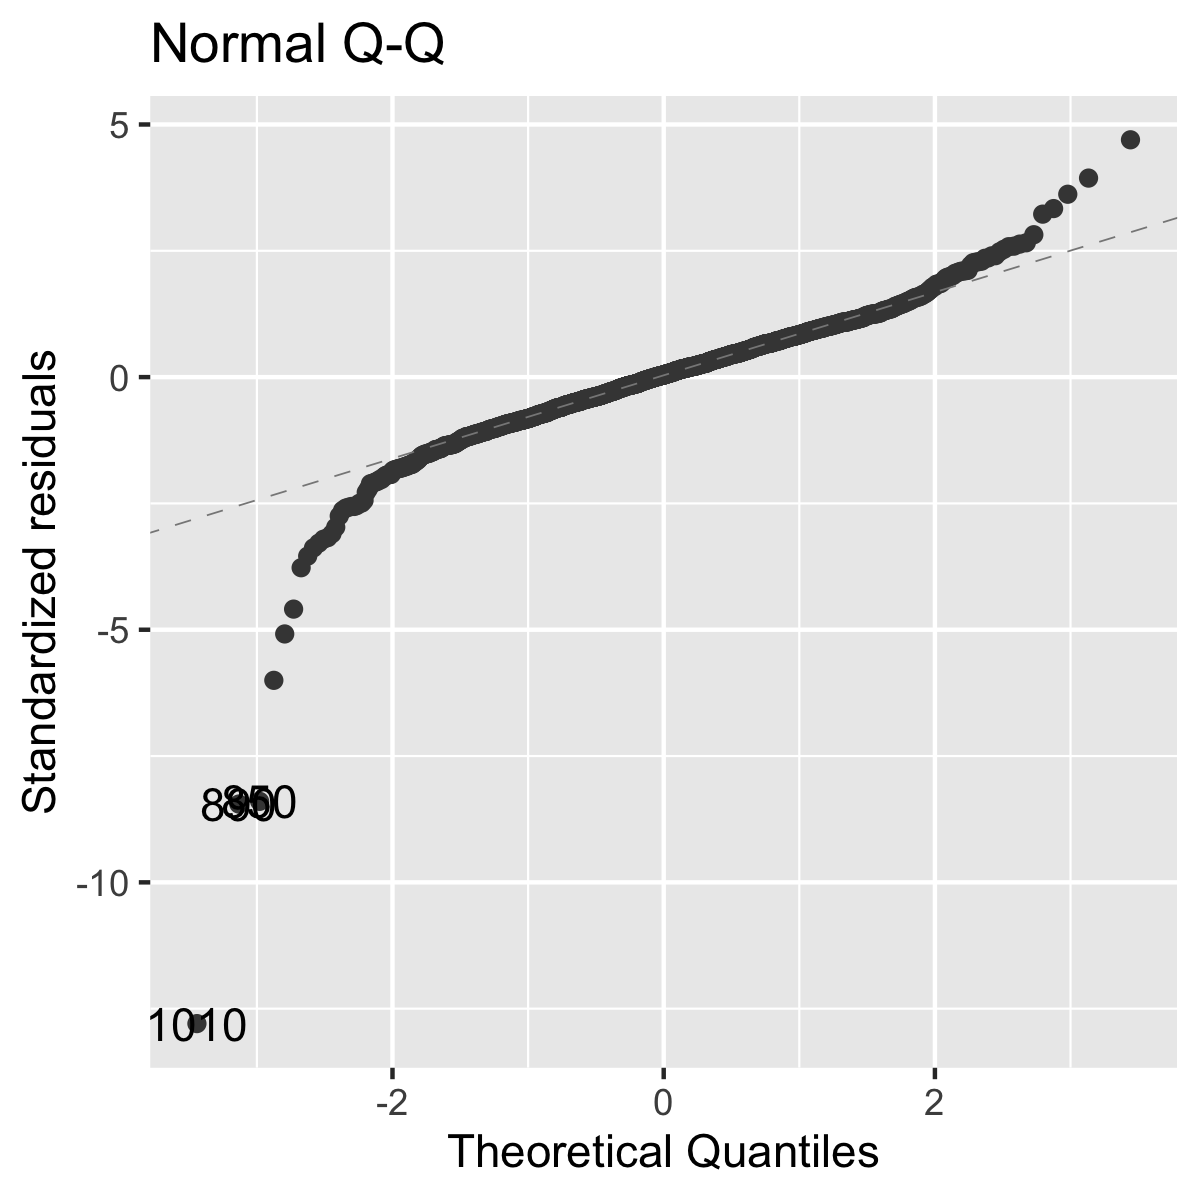
\includegraphics[width=0.49\linewidth]{plot6} 

}

\caption{Residual vs Fitted and QQplot for log-linear transformed model}\label{fig:unnamed-chunk-7}
\end{figure}

\begin{figure}[h]

{\centering 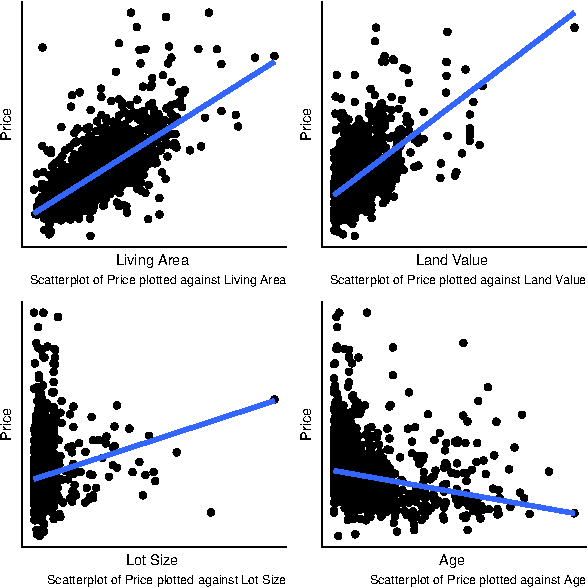
\includegraphics[width=0.75\linewidth]{Report_files/figure-latex/unnamed-chunk-8-1} 

}

\caption{Scatterplots of independent variables vs price selected from stepwise selection model}\label{fig:unnamed-chunk-8}
\end{figure}

\begin{figure}[h]

{\centering 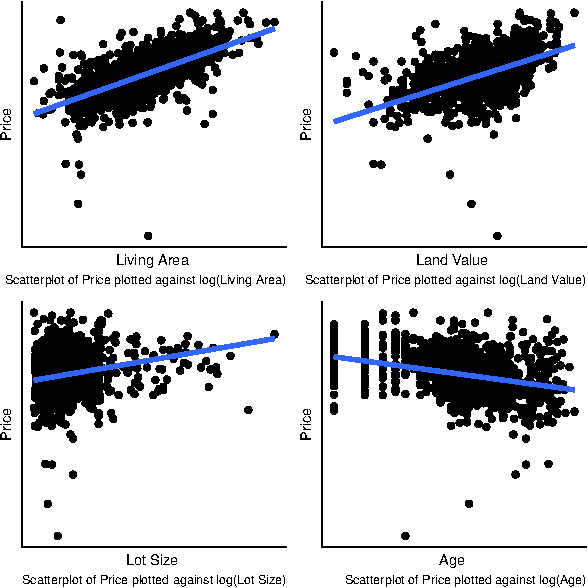
\includegraphics[width=0.75\linewidth]{Report_files/figure-latex/unnamed-chunk-9-1} 

}

\caption{Scatterplots of independent variables vs price selected from the final model}\label{fig:unnamed-chunk-9}
\end{figure}

%\showmatmethods


\bibliography{pinp}
\bibliographystyle{jss}



\end{document}
